%% 
%% Copyright 2007-2020 Elsevier Ltd
%% 
%% This file is part of the 'Elsarticle Bundle'.
%% ---------------------------------------------
%% 
%% It may be distributed under the conditions of the LaTeX Project Public
%% License, either version 1.2 of this license or (at your option) any
%% later version.  The latest version of this license is in
%%    http://www.latex-project.org/lppl.txt
%% and version 1.2 or later is part of all distributions of LaTeX
%% version 1999/12/01 or later.
%% 
%% The list of all files belonging to the 'Elsarticle Bundle' is
%% given in the file `manifest.txt'.
%% 
%% Template article for Elsevier's document class `elsarticle'
%% with harvard style bibliographic references

%\documentclass[12pt]{elsarticle}

%% Use the option review to obtain double line spacing
%% \documentclass[preprint,review,12pt]{elsarticle}

%% Use the options 1p,twocolumn; 3p; 3p,twocolumn; 5p; or 5p,twocolumn
%% for a journal layout
%% \documentclass[final,1p,times]{elsarticle}
%% \documentclass[final,1p,times,twocolumn]{elsarticle}
%% \documentclass[final,3p,times]{elsarticle}
\documentclass[final,5p,times,twocolumn]{elsarticle}
%% \documentclass[final,5p,times]{elsarticle}
%% \documentclass[final,5p,times,twocolumn]{elsarticle}

%% For including figures, graphicx.sty has been loaded in
%% elsarticle.cls. If you prefer to use the old commands
%% please give \usepackage{epsfig}

%% The amssymb package provides various useful mathematical symbols
\usepackage{amssymb,amsmath}
%\newcommand{\diff}[3]{\frac{\partial^{#3}#1}{\partial #2^{#3}}}
\newcommand{\diff}[2]{\frac{\partial#1}{\partial #2}}
\newcommand{\Diff}[3]{\frac{d^{#3}#1}{d #2^{#3}}}

\newcommand{\bfm}[1]{\mathchoice {\mbox{\boldmath$\displaystyle#1$}}
    {\mbox{\boldmath$\textstyle#1$}}
    {\mbox{\boldmath$\scriptstyle#1$}}
    {\mbox{\boldmath$\scriptscriptstyle#1$}}}


\usepackage[dvipsnames]{xcolor}
\newcommand{\grant}[1]{\textcolor{CornflowerBlue}{#1}}

\def\nb{\boldsymbol{n}}
\def\rhob{\boldsymbol{\rho}}
\def\varrhob{\boldsymbol{\varrho}}
\def\thetab{\boldsymbol{\theta}}
\def\varthetab{\boldsymbol{\vartheta}}
\def\etab{\boldsymbol{\eta}}
\def\Lambdab{\boldsymbol{\Lambda}}
\def\Gammab{\boldsymbol{\Gamma}}
\def\ab{\boldsymbol{a}}
\def\bb{\boldsymbol{b}}
\def\cb{\boldsymbol{c}}
\def\eb{\boldsymbol{e}}
\def\qb{\boldsymbol{q}}
\def\Qb{\boldsymbol{Q}}
\def\Jb{\boldsymbol{J}}
\def\kb{\boldsymbol{k}}
\def\lb{\boldsymbol{l}}
\def\rb{\boldsymbol{r}}
\def\sb{\boldsymbol{s}}
\def\ub{\boldsymbol{u}}
\def\vb{\boldsymbol{v}}
\def\wb{\boldsymbol{w}}
\def\xb{\boldsymbol{x}}
\def\yb{\boldsymbol{y}}
\def\zb{\boldsymbol{z}}
\def\xib{\boldsymbol{\xi}}
\def\Fb{\boldsymbol{F}}
\def\Mb{\boldsymbol{M}}
\def\Tb{\boldsymbol{T}}
\def\Xb{\boldsymbol{X}}
\def\Wb{\boldsymbol{W}}
\def\Yb{\boldsymbol{Y}}

\def\grad{\nabla}
\def\div{\nabla \cdot}
\def\lap{\Delta}

\def\d{\displaystyle} \def\t{\textstyle} \def\scr{\scriptstyle}
\def\sscr{\scriptscriptstyle} \def\sp{\vspace{2mm}}

\def\lap{\Delta}
\def\eps{\varepsilon}

\def\kbT{k_\mathrm{B} T}

\def\RR{\mathbb{R}} \def\NN{\mathbb{N}} \def\ZZ{\mathbb{Z}}
\def\EE{\mathbb{E}}\def\PP{\mathbb{P}}

\newcommand{\ddt}{\frac{\partial}{\partial t}}
\newcommand{\ddx}{\frac{\partial}{\partial x}}
\newcommand{\avg}[1]{\left\langle #1 \right\rangle}
%\newcommand{\dbar}{{\mkern3mu\mathchar'26\mkern-12mu d}}

\def\<{\langle} \def\>{\rangle}

\DeclareRobustCommand{\ran}{\operatorname*{ran}}
\DeclareRobustCommand{\supp}{\operatorname*{supp}}
\DeclareRobustCommand{\argmin}{\operatorname*{argmin}}
\DeclareRobustCommand{\sign}{\operatorname*{sign}}

%% The amsthm package provides extended theorem environments
%% \usepackage{amsthm}
%% The lineno packages adds line numbers. Start line numbering with
%% \begin{linenumbers}, end it with \end{linenumbers}. Or switch it on
%% for the whole article with \linenumbers.
%% \usepackage{lineno}

\journal{Current Opinion in Solid State and Materials Science}

\begin{document}

\begin{frontmatter}

%% Title, authors and addresses

%% use the tnoteref command within \title for footnotes;
%% use the tnotetext command for theassociated footnote;
%% use the fnref command within \author or \address for footnotes;
%% use the fntext command for theassociated footnote;
%% use the corref command within \author for corresponding author footnotes;
%% use the cortext command for theassociated footnote;
%% use the ead command for the email address,
%% and the form \ead[url] for the home page:
%% \title{Title\tnoteref{label1}}
%% \tnotetext[label1]{}
%% \author{Name\corref{cor1}\fnref{label2}}
%% \ead{email address}
%% \ead[url]{home page}
%% \fntext[label2]{}
%% \cortext[cor1]{}
%% \affiliation{organization={},
%%             addressline={},
%%             city={},
%%             postcode={},
%%             state={},
%%             country={}}
%% \fntext[label3]{}

\title{Sampling thermodynamic ensembles of molecular systems with generative neural networks: Will integrating physics-based models close the generalization gap?}

%% use optional labels to link authors explicitly to addresses:
\author[label1,label2]{Grant M. Rotskoff}
\affiliation[label1]{organization={Department of Chemistry, Stanford University},
            %addressline={Keck Science Building},
            city={Stanford},
            postcode={94305},
            state={CA},
            country={USA}}
%%
\affiliation[label2]{organization={Institute for Computational and Mathematical Engineering},
            %addressline={},
            city={Stanford},
            postcode={94305},
            state={CA},
            country={USA}}

% \affiliation{organization={Stanford University},%Department and Organization
%             addressline={}, 
%             city={},
%             postcode={}, 
%             state={},
%             country={}}

\begin{abstract}
If the promise of generative modeling techniques is realized, it may fundamentally change how we carry out molecular simulation.
The suite of techniques and models collectively termed ``generative AI'' includes many different classes of models, built for varied types of data, from natural language to images.
Recent advances in the machine learning literature that construct ever better generative models, though, do not contend with the challenges unique to complex, molecular systems. 
To generate a statistically likely molecular configuration, many correlated degrees of freedom must be sampled together, while also satisfying the strong constraints of chemical physics. 
Recent efforts to develop generative models for biomolecular systems have shown spectacular results in some cases---nevertheless, some simple systems remain out of reach with our present methodology.
Arguably, the central concern is data-efficiency: we should aim to train models that can meaningfully extrapolate from their training data and hence facilitate discovery.
In this review we discuss methods and future directions for directly incorporating physics-based models into generative neural networks, which we believe is a crucial step for addressing the limitations of the current toolkit.
\end{abstract}

% %%Graphical abstract
% \begin{graphicalabstract}
% %\includegraphics{grabs}
% \end{graphicalabstract}

% %%Research highlights
% \begin{highlights}
% \item Research highlight 1
% \item Research highlight 2
% \end{highlights}

% \begin{keyword}
% %% keywords here, in the form: keyword \sep keyword

% %% PACS codes here, in the form: \PACS code \sep code

% %% MSC codes here, in the form: \MSC code \sep code
% %% or \MSC[2008] code \sep code (2000 is the default)

% \end{keyword}

\end{frontmatter}

%% \linenumbers

%% main text
\section{Introduction and background}
\label{sec:intro}


Supervised machine learning has a rich history in the chemical sciences~\cite{lederberg_applications_1969}. 
For many decades, fitting linear and nonlinear regression models to experimental data has been a central modality of data-driven science.
In the last decade, both the complexity and expressiveness of the available models have grown rapidly: as the library of neural network architectures expanded, models that are well-calibrated for chemical and dynamical data have been widely and enthusiastically deployed in experimental and theoretical chemistry~\cite{}. 
While these algorithmic innovations have spurred substantive progress in cheminformatics~\cite{mater_deep_2019} and the physical sciences more broadly~\cite{carleo_machine_2019}, one cannot discount the formative role played by increasingly powerful computational resources~\cite{amodei_ai_2018} alongside sophisticated and reliable software for automatic differentiation and optimization~\cite{paszke_pytorch_2019, bradbury_jax_2018, broughton_tensorflow_2020}. 
Together, these developments have led to an active community of research designing ever better networks, optimization strategies, and data curation to further improve the performance of data driven models.

A comparably new modeling paradigm is emerging alongside the developments in supervised learning due to the extraordinary developments in generative modeling.
Often called ``unsupervised learning'' as a contrast with regression or classification tasks on labelled data, generative models seek to directly emulate data.
For the purposes of this review, we will define a generative model to be any model that is parameterized to draw samples from a target probability distribution.
Information about a target probability distribution is either accessible through a data set of samples drawn from the distribution or, alternatively, through the unnormalized statistical likelihood function, which for a Gibbs-Boltzmann distribution is simply the energy.  
Generative models have attracted enormous attention for applications outside of science, such as text-to-image generation with denoising diffusion models~\cite{song_score-based_2022,ho_denoising_nodate} and autoregressive text generation with large language models (LLMs)~\cite{vaswani_attention_2017}. 
The natural question, of course, is whether or not these approaches can amplify and accelerate scientific inquiry in the chemical context.

In this review, we seek to articulate the potentialities and challenges of using generative models to sample finite temperature equilibrium probability distributions of chemical systems in the condensed phase.
We emphasize that this task is considerably different from, for example, protein structure prediction using alphaFold~\cite{jumper_highly_2021}, which predicts the crystal structure but does not capture molecular fluctuations.
Perhaps the defining challenge facing the generative modeling paradigm is \emph{generalization}: in many complex scientific tasks, large repositories of training data simply do not exist and generative models must instead be built from smaller data sets than those used for image generation applications~\cite{dalle} or LLMs~\cite{vaswani_attention_2017,gpts}.
If a generative model can only effectively sample molecular configurations that are very close to those provided in an initial dataset, then little useful information can be gained from sampling the generative model. 
Nevertheless, researchers are actively building strategies to augment data, improve transferrability, and enhance generalization by integrating generative models into enhanced sampling schemes already widely used in molecular simulation.

To provide a comprehensive overview of the challenges and opportunities afforded by generative models, we will first review current modeling paradigms, neural network architectures, and training approaches, without specializing to molecular systems. 
We will then discuss efforts to incorporate \emph{physical inductive bias}, that is, natural physical invariance and equivariance into generative neural networks, which promises to improve the quality of the generated samples and reduce training effort.
Our central focus will be on the question generalization and we will discuss several distinct strategies that seek to improve the capacity of these models for discovery, a question that remains formative for this new and developing field.


\section{Generative modeling for molecular systems}

For a molecular system in thermal equilibrium at constant temperature, volume, and particle number, we know from elementary statistical mechanics~\cite{chandler_introduction_1987} that the probability density of a given configuration can be written as,
\begin{equation}
    \varrho_{\rm eq}(\xb) = Z^{-1} e^{-\beta U(\xb)},
    \label{eq:rhoeq}
\end{equation}
where $\beta=1/(k_{\rm B} T)$, $U$ is the potential energy function for the system, and $Z = \int_{\Omega} e^{-\beta U(\xb)} d\xb$ is the normalization constant for the distribution, also called the partition function. 
Of course, it is not possible to evaluate $\varrho_{\rm eq}$ directly because the partition function is ``intractable'', requiring that we compute a high-dimensional integral which is typically impossible.

Because we have accurate models of the energy $U$ from either electronic structure methods or classical approximations collectively referred to as molecular force fields~\cite{case_amber_2005, vanommeslaeghe_charmm_2010}, we usually draw samples from~\eqref{eq:rhoeq} with Markov chain Monte Carlo (MCMC) sampling algorithms.
Access to a collection of configurations allows us to estimate observable properties of the system by evaluating an ``empirical expectation'' or sample average,
\begin{equation}
\begin{aligned}
    \avg{\mathcal{A}} &= Z^{-1} \int_{\Omega} \mathcal{A}(\xb) e^{-\beta U(\xb)} d\xb, \\
    &\approx \frac1n \sum_{i=1}^n \mathcal{A}(\xb_i), \quad \xb_i \sim \varrho_{\rm eq},
    \label{eq:avg}
\end{aligned}
\end{equation}
for any observable function $\mathcal{A}.$
In principle, estimating \eqref{eq:avg} is straightforward, requiring only a direct MCMC simulation or a molecular dynamics (MD) simulation in which the samples have been appropriately ``metropolized'' to ensure Boltzmann statistics~\cite{}. 
In practice, such estimates rarely converge quickly because molecular systems often have metastable probability distributions, as illustrated in Fig.~\ref{fig:metastable}. 
The amount simulation time and hence computational effort required for MD or MCMC to ``mix'' between the two metastable configurations is simply prohibitive in many processes of interest~\cite{lelievre_free_2010}.

Generative models, which seek to directly approximate $\varrho_{\rm eq}$ and sample efficiently from it, do not suffer from the issue of slow mixing because each new sample is statistically uncorrelated from the last.
However, we must optimize a parametric model to approximate the target probability distribution, which itself incurs a computational cost.
Supposing that we build a generative model with parameters $\theta$ for which we can compute exactly the normalized probability density of the samples we generate $\rho_{\theta}$, then the associated Metropolis-Hastings acceptance criterion a newly proposed configuration in a Markov chain $\xb_0, \dots, \xb_k$ is~\cite{gabrie_adaptive_2022},
\begin{equation}
    \textrm{acc}(\xb_k \to \xb_{k+1}) = \min \left[ 1, \frac{\varrho_{\rm eq}(\xb_{k+1})\rho_{\theta}(\xb_{k}) }{\varrho_{\rm eq}(\xb_{k})\rho_{\theta}(\xb_{k+1}) }\right].
\end{equation}
Importantly, this scheme correctly accounts for the proposal distribution and has the transparent outcome that, if the generative model is identical to the Boltzmann distribution, the acceptance probability is unity. 
This discussion assumes, of course, that it is possible to efficiently build a generative model that i) accurately approximates a given target distribution and ii) allows accurate or exact evaluation of $\rho_{\theta}$ for an arbitrary sample. 
Neither of these assumptions should be taken for grant: we will focus primarily on these questions in the present review.


In general, there are two distinct strategies for building a generative model to represent a Boltzmann distribution: \emph{training with data} and \emph{training with energy}, which we discuss in detail below. 

\subsection{Models trained purely with data}

The most widely used strategies for building generative models require training data.
In some sense, when training with data, these problems become supervised learning problems in which a probabilistic model is trained to recapitulate the data and smoothness is exploited to obtain ``nearby'' configurations.
Many modern generative neural networks were designed for image data, where, as we can intuitively recognize, small perturbations do not typically affect our ability to interpret the result. 
However, this is not the case for molecular systems: a single particle-particle overlap or a violation of chemical bonding rules can be catastrophic. 

In the following discussion, we will focus on two closely related generative modeling strategies, namely, denoising diffusion probabilistic models, which we will simply call \emph{diffusion models}, and flow matching models~\cite{lipman_flow_2022, albergo_building_2022, albergo_stochastic_2023} which are also known as stochastic interpolants.  
There are many classes of generative models that we choose not to discuss here, including generative adversarial networks~\cite{goodfellow_generative_2014} and restricted Boltzmann machines~\cite{} because, while powerful, these models are lesser used in the applications of interest to this review. 

When discussing models trained with data, we will assume that we are given a data set consisting of $n$ points, denoted $\mathcal{D} = \{ \xb_i \}_{i=1}^n$.
While the frameworks are far more general, the applications we have in mind are those for which each point $\xb_i$ is a molecular configuration and is distributed according to a Boltzmann distribution, i.e., $\xb_i \sim \varrho_{\rm eq}.$

\subsubsection{Denoising diffusion models}

Diffusion models were initially developed in Ref.~\cite{sohl-dickstein_hamiltonian_2012} using a theoretical framework based on time-reversed dynamics that has its origins in the nonequilibrium statistical mechanics literature~\cite{crooks_entropy_1999}. 
At a high level, the idea of diffusion models to define a stochastic process in which we progressively transform samples from a data set into statistical noise.
Among the mostly widely used approaches is to simulate an Ornstein-Uhlenbeck process starting from a data point $\xb$.
Explicitly, for some time interval $[0, T]$, we use
\begin{equation}
    d\Xb_t = - \beta(t) \Xb_t dt + \sqrt{2 \beta(t)} d\Wb_t; \quad \Xb_0 = \xb.
    \label{eq:ou}
\end{equation}
Because an Ornstein-Uhlenbeck process converges exponentially fast to Gaussian distribution, for sufficiently large times $T$, the samples are nearly indistinguishable from Gaussian random variables. 

The key insight underlying diffusion models is that, with the collection of trajectories obtained by the noising dynamics~\eqref{eq:ou}, we can learn a representation of the time-reversal of this dynamics and convert noise into samples that resemble the target distribution.
In fact, Fokker-Planck equation associated with the stochastic process defined in~\eqref{eq:ou} has an exact time-reversal~\cite{anderson_reverse-time_1982,song_score-based_2022} which leads to the unknown reverse process,
\begin{equation}
    d\tilde{\Xb}_t = -\beta(t)[\tilde{\Xb}_t + \nabla \log \rho_t(\tilde{\Xb}_t)] dt + \sqrt{2 \beta(t)} d\tilde{\Wb}_t; \quad \tilde{\Xb}_0\sim \mathcal{N}(0,\rm{Id}).
    \label{eq:revou}
\end{equation}
A generative model is constructed by approximating the ``score'' of the intermediate time distributions, $\nabla \log \rho_t$, using a neural network $s(\xb, t; \theta)$.
This procedure is known as score-matching~\cite{song_score-based_2022} and a converged score function enables sampling from the data distribution simply by simulating~\eqref{eq:revou}.
\grant{write the objective and emphasize its data dependence here}
\grant{
Of course, the intermediate distributions $\rho_t$ and the score function $\nabla \rho_t$ are not easy to estimate, but an objective function that requires only conditional expectations can be constructed to efficiently approximate $s$.
TODO: comments about constraints on the resulting SDEs
}
Diffusion models have already been embraced in a variety of contexts, and while there are several different formalisms (discrete time~\cite{ho_denoising_nodate}, continuous time~\cite{song_score-based_2022,vroylandt_likelihood-based_2022}) all these approaches share in common a dynamics that flows samples from a data set to a tractable distribution and a data-dependent parameterization of the inverse dynamics.
See ~\cite{} for a comprehensive overview. 

Diffusion models have a variety of advantages that make them suitable for working with physical systems. 
One important aspect of the generative process is that the physical invariants can be directly incorporated into the score function.
For example, ~\cite{schneuing_structure-based_2022,weiss_guided_2023} introduced parameterizations of the score that are equivariant with respect to rotations, translations invariant, and permutation invariant for identical atoms.
Ensuring that physical invariances are respected is believed to aid data-efficiency and improve generalization, and there is some empirical evidence to support this belief~\cite{sannai_improved_2021}.
Furthermore, it is possible incorporate physics-based regularizations~\cite{zheng_towards_2023}, which could be useful for treating systems with hard-core repulsive interactions or long-ranged Coulombic interactions.

Ensuring detailed balance within a Metropolis-Hastings scheme requires accounting for asymmetry in the proposal distribution~\cite{frenkel_understanding_2002}.
For generative models, this means that the acceptance criterion for an MCMC proposal is simply
\begin{equation}
    \textrm{acc}(\xb_{k} \to \xb_{k+1}) = \min \left[ 1, \frac{\hat{\rho}(\xb_{k})}{\hat{\rho}(\xb_{k+1})} e^{-\beta \Delta U(\xb_{k+1},\xb_k)} \right].
    \label{eq:mhacc}
\end{equation}
Because the normalization constant cancels in the ratio of generative model probabilities in \eqref{eq:mhacc}, we need only the unnormalized statistical weights associated with the samples, typically called the likelihood in the Bayesian context.
\grant{To compute likelihoods for samples generated by the denoising diffusion model, one needs to integrate an ordinary differential equation that...
comments on hutchinson trace estimator...
}

\begin{figure*}
    \centering
    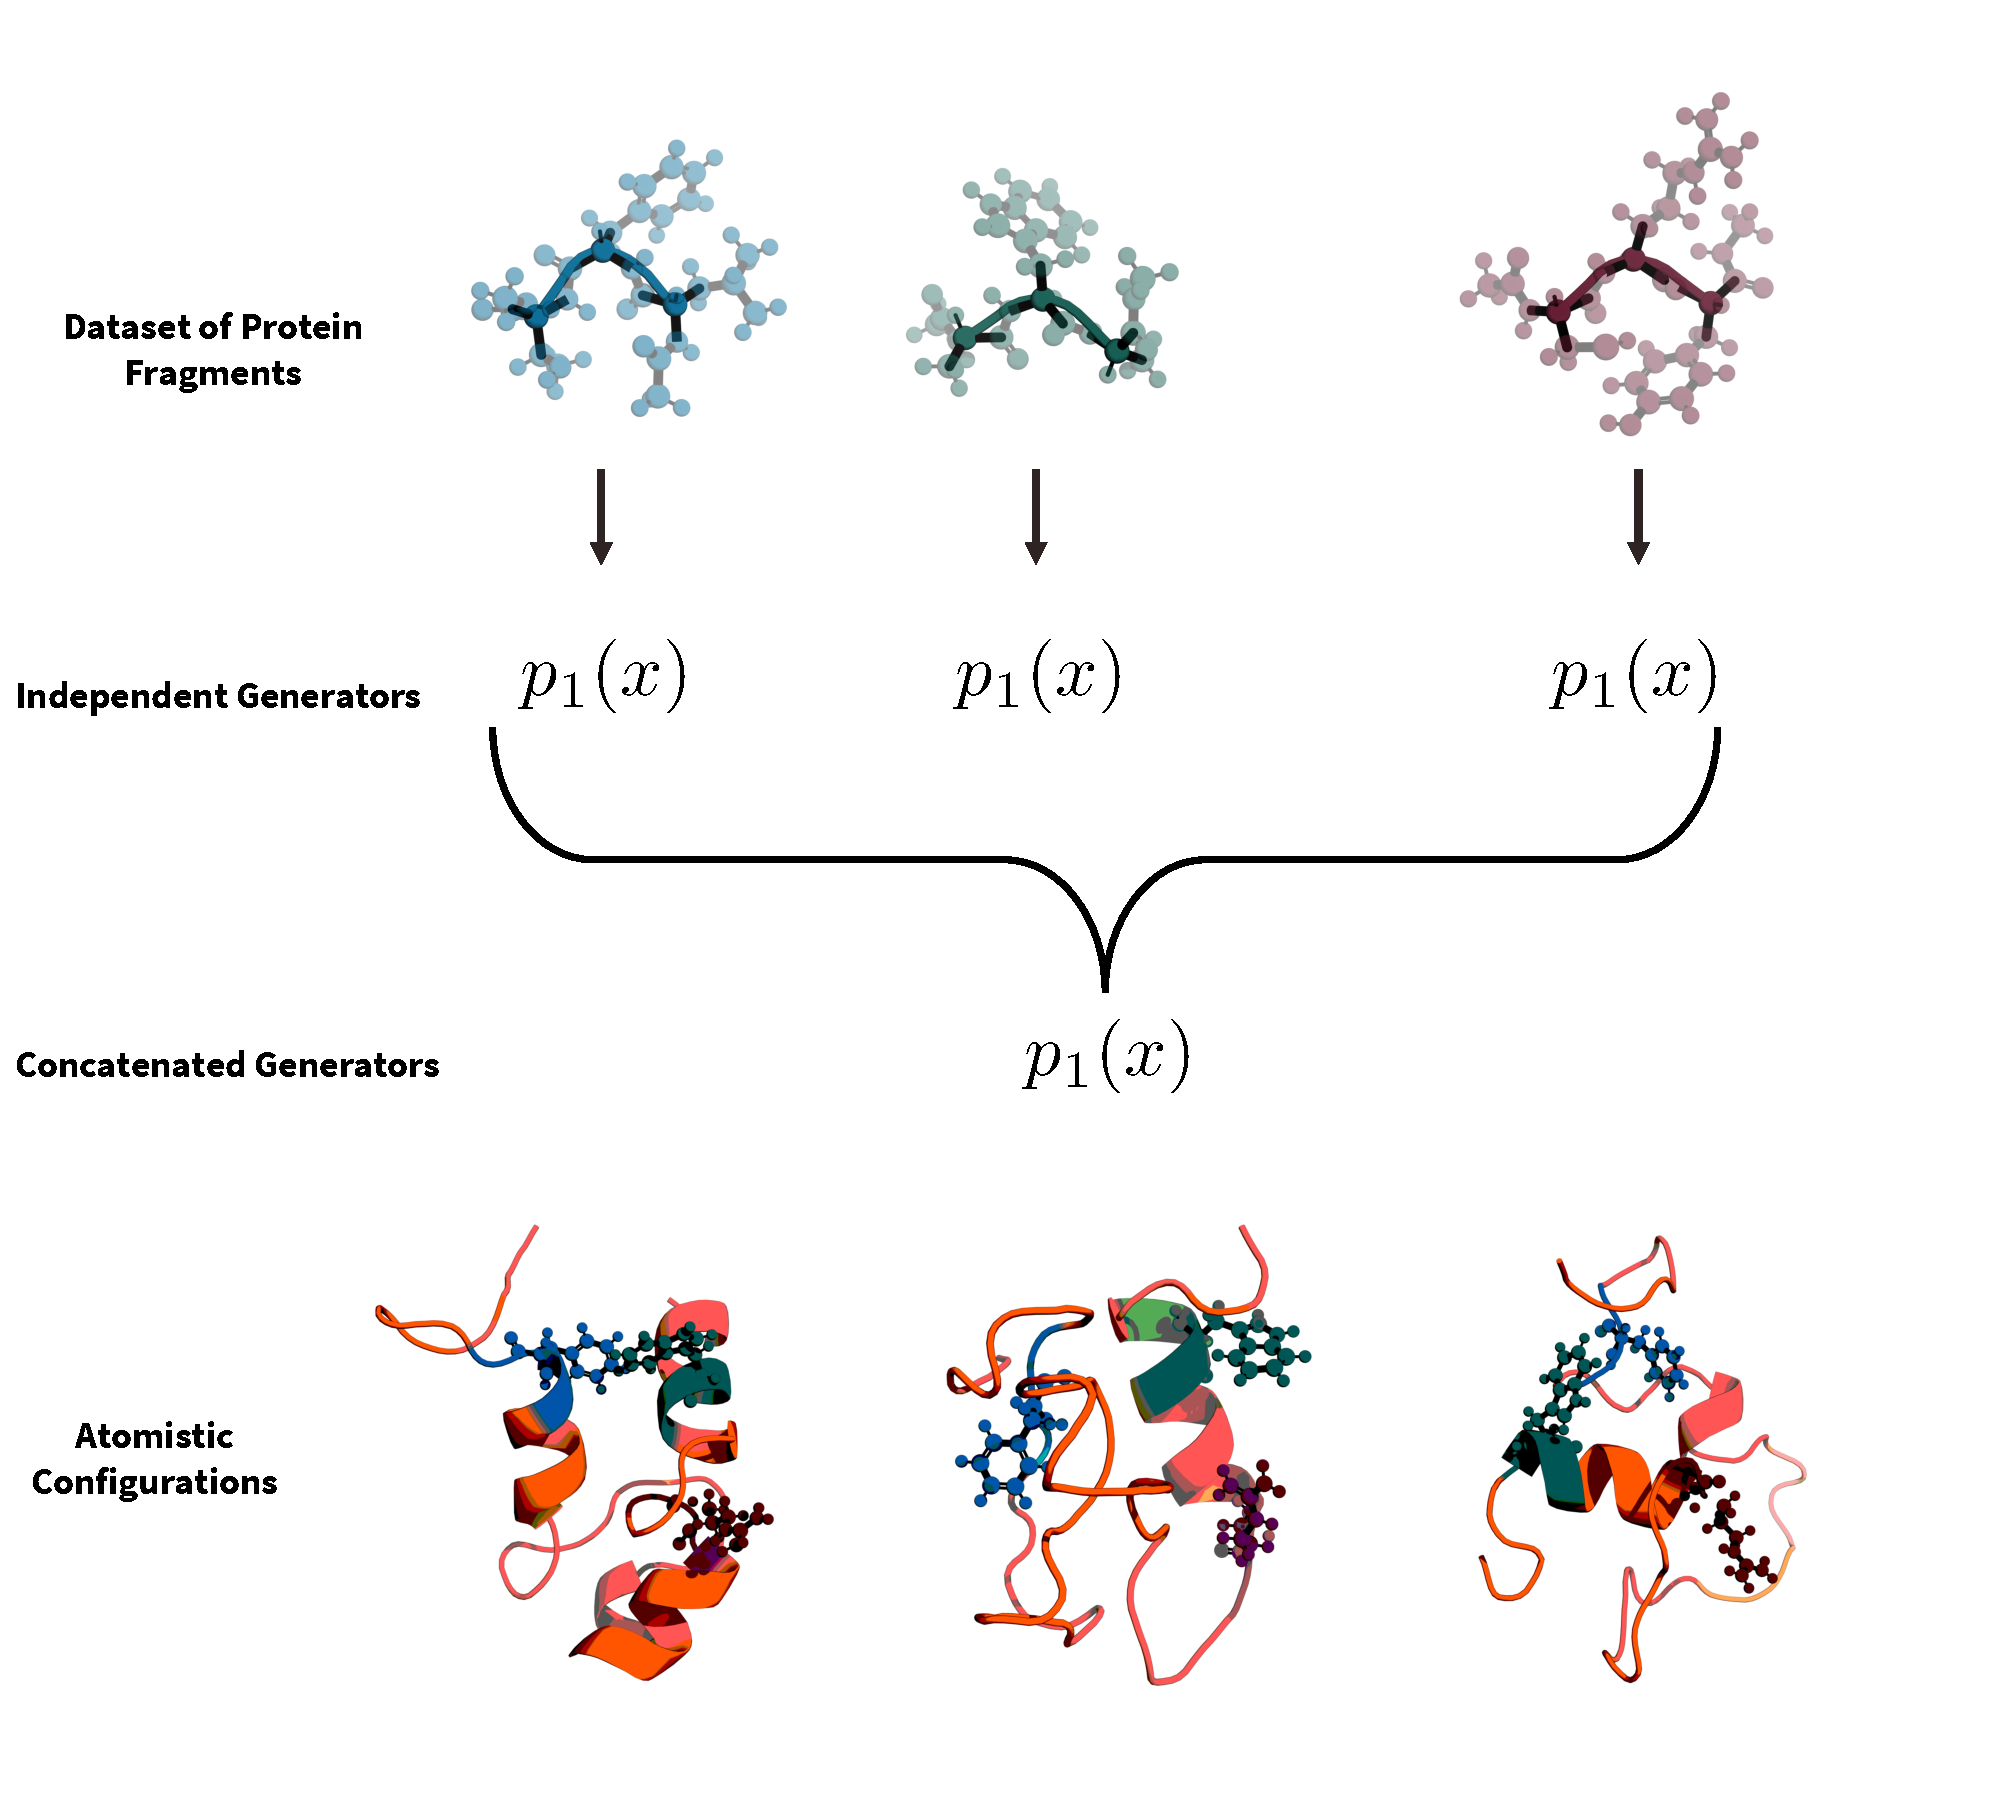
\includegraphics[width=0.6\linewidth]{modular_fig.pdf}
    \caption{Caption}
    \label{fig:enter-label}
\end{figure*}

\subsubsection{Flow-based models}

The idea of transforming samples from an ``easy'' distribution, like a Gaussian, into intricately structured random variables has also motivated more direct approaches.
Normalizing flows~\cite{tabak_density_2010,rezende_variational_2015} seek to transform a tractable initial distribution into samples with high probability in the target distribution with a single map.
Such a transformation, which depends on optimizable parameters $\theta$ and we denote $T_{\theta}$, generates samples by ``pushing forward'' samples from the initial distribution. 
Importantly, normalizing flows are chosen to be invertible functions, meaning that the probability of samples generated by transforming noise with $T_{\theta}$ can be evaluated exactly.
Explicitly,
\begin{equation}
\begin{aligned}
    \xb &= T_{\theta}(\zb) \quad \zb \sim \rho_0, \\
    \hat \rho_\theta(\xb) &= \rho_0(T_{\theta}^{-1}(\xb)) |\nabla T_{\theta}^{-1}(\xb)|,
\end{aligned}
\end{equation}
where $\rho_0$ is the tractable initial distribution and the notation $|\nabla f|$ denotes the determinant of the Jacobian, which arises simply from change of variables. 
Among the most widely used normalizing flow architectures are RealNVP coupling layers~\cite{dinh_density_2017} and rational quadratic splines~\cite{}.
The requirement of invertibility is a strong constraint and the currently available normalizing flow models can be challenging to optimize~\cite{}.

An alternative strategy for building invertible maps exploits the \emph{neural ordinary differential equations}~\cite{chen_neural_2018} framework.
The free-form Jacobian of continuous dynamics (FFJORD) algorithm exploits the classical adjoint state method~\cite{} to optimize an parametric ordinary differential equation using a maximum likelihood loss function. 
In some examples, normalizing flows built with continuous-time ODEs add significant flexibility to models compared with those built on coupling layers which have a restricted functional form.
This approach is, however, limited computationally due to the requirement that the ODE be solved numerically for sample generation. 
Furthermore, computing exact likelihoods is not tractable for high-dimensional systems because the trace of the Jacobian matrix requires $\mathcal{O}(d^2)$ operations in dimension $d$ at every step of the ODE solve.
To mitigate this, the trace is typically estimated using the Hutchinson trace estimator~\cite{hutchinson}, but the variance can be problematic. 

Recent works that seek to extend and enhance the framework of continuous normalizing flows (cf. Sec.~\ref{sec:nfs}) have introduced flow matching~\cite{peluchetti_non-denoising_2022,peluchetti_diffusion_2023,lipman_flow_2022} or stochastic interpolants~\cite{albergo_building_2022, albergo_stochastic_2023}.
In this generative modeling framework, the transformation between the tractable Gaussian distribution and the target is first built from a library of simple interpolating functions~\cite{albergo_stochastic_2023}, 
\begin{equation}
    I(x_0, x_1, t) = \alpha(t) x_0 + \beta(t) x_1 + \gamma(t) z,
\end{equation}
where $\alpha$ and $\beta$ are such that 
The function $\gamma$ is such that .... and $z$ is a Gaussian random variable.

These models share many commonalities with diffusion models, but differ in several potentially important ways.
For diffusion models, the noising dynamics~\eqref{eq:ou} does not completely lose memory of its initial condition in a finite time, meaning that the noise samples are not exactly Gaussian distributed.
Because flow-matching models learn a transformation directly between a noise distribution and the target distribution, no approximation is needed to use these models as generative models. 
Furthermore, the relatively implicit objective function used in score-matching constrains choice the noising dynamics: it will be computationally efficient only if~\eqref{eq:ou} is linear.
Flow-matching models, on the other hand, are optimized using regression directly on the learned velocity field. 
For modeling physical systems, this means that natural regularization terms and constraints can be directly incorporated into the entire generative process. 
While these models have not yet been used widely for physical data, these properties suggest that they could provide a productive avenue for sampling molecular systems. 

However, like diffusion models, likelihood estimation is difficult. 
Computing the likelihood of samples generated from the learned velocity field requires an integral, 
\begin{equation}
    \int \nabla \cdot b 
\end{equation}
which will not be tractable in high-dimensional systems.


\subsubsection{Generic challenges with data-based training}

- we know it works and is stable, but what if the distributions are rugged
- we don't want situations where the available data is too small


\subsection{Models trained with statistical likelihoods}

Because computing likelihoods is straightforward by construction for normalizing flow models, it is also possible to use a maximum likelihood approach to train the model. 
To do, we use the ``forward'' KL divergence as the loss function
\begin{equation}
    D_{KL}(\hat\rho_{\theta} \| \varrho_{\rm eq}) = \int \log \frac{\hat\rho_{\theta}(\xb)}{\varrho_{\rm eq}(\xb)} \hat\rho_{\theta}(\xb) d\xb.
    \label{eq:energy_kl}
\end{equation}
The appeal of this training modality is that it requires, in principle, \emph{no data}.
The samples are generated by pushing forward random variables from the tractable base distribution $\rho_0$ with the parametric map $T_{\theta}$.
The objective \eqref{eq:energy_kl}

- when there's no data, a common case, one instead samples directly from the model and compares its likelihood to the target
- this requires more specialized technology, because likelihood computations are difficult
- for ddpms and flow based models, it can be done in principle but requires the use of estimators that have high variance
- normalizing flows, discussed in the next section, solve this problem by restricting the models

- the main problem with energy based training is mode collapse
- a variety of works have introduced different models / training procedures to mitigate, but it seems fundamental 
- 


\section{Direct density estimation with normalizing flows}

- energy based training more natural, but suffers from mode collapse
- data based training more interpolative, so less to learn from the model
- Boltzmann generators were an unmitigated disaster that misled everyone and are still confusing the literature
- recent works show that augmenting with additional mcmc steps helps

\subsection{Adapting normalizing flow models for physical systems}

The empirically observed challenges with adapting normalizing flows to complex, multimodal target data has initiated a line of research that seeks to better parameterize invertible models for physical data. 
Here, we review three distinct strategies for incorporating a physical inductive bias into the model: i) informed probability 

- informed based measures

- permutation symmetry and periodic boundary conditions

- recent works with diffusion models integrating PINN loss terms

\section{Augmenting mode discovery with coarse-grained models}

The dual problem of mode collapse and lack of data requires fundamentally different approaches for building generative models to sample thermodynamic ensembles.
Several recent works have sought to enhance sampling by carrying out dynamics in a ``latent'' space and subsequently recovering the atomistic molecular configuration using a generative model.
Perhaps the earliest among these works is Sidky et al.~\cite{sidky_molecular_2020}, which builds a generative adversarial network from molecular dynamics trajectory data. 
Among the 

\section{Enhancing sampling with normalizing flows}

\section{Challenges and outlook}

 \bibliographystyle{elsarticle-num-names} 
 \bibliography{references}

\end{document}